\chapter{Parallel computation of the exposure map}
\label{appendix:exposure}

Long calculation time for the exposure calculation comes from 
two matrix transformations to accumulate the LAT exposure 
when the Earth is in the FoV.
% Since the FT2 or spacecraft log file is
% recorded in the position and all metadata.

For each step time, 
the transformation matrix is calculated from the 
information of spacecraft orientation.
After that, each nadir angle 
represented in equatorial coordinates (Equation \ref{eq:def_r0})
is transformed into angles in the plane
of detector (Equation \ref{eq:def_r0_to_rp}).
Hence, we can calculate the exposure for a given nadir angle
by summing the LAT exposure time multiplied with 
the effective area for the corresponding incidence angle and energy.

The resolution of the exposure map impacts the computational time.
% There is one thing that could be used to approximate the 
% complexity of the code which is the resolution of the exposure map.
Assuming that there are $M$ bins in $\theta_\text{NADIR}$ axis
and $N$ bins in $\phi_\text{NADIR}$ axis.
It costs $\mathcal{O}(MN)$ multiplied
% It will cost $\mathcal{O}(MN)$ multiply
by the complexity of two 
transformation matrices to compute a single exposure map.
This complexity will be multiplied by 50 times 
since we have 50
energy bins.
% bins that have their own specific mean energy 
% which affects the effective area.


The first version of Python code takes around 1435 seconds to finish 
one week of FT2 data.
% There are 531 weeks to calculate, then 
% it will take around 9 days to finish this task.
In addition, the matrix transformation
already uses Numpy for
% is already used Numpy for
all matrix operations which means that the plain Python code 
likely to takes longer than this speed. In the meantime, using 
serial a serial C++ code takes around 12 seconds to finish 
the workload
of 1-week data, showing $\sim120$ times
faster for the compiling language.
% of a single week. Meaning that the calculation time 
% is $\sim$120 times faster from the compiling language.

The parallel code is implemented in the C++ programming language 
with Message Passing Interface (MPI). We use Master-Slave techniques
to fully utilize the CPU resources where the master process 
is monitoring and sending tasks to all workers.
Only one master process is needed to allow
% Consequently, there is only one master process and allows
the program to scale horizontally (multi-node scaling)
by adjusting the number of slave processes. 

\begin{figure}[h]
    \centering
    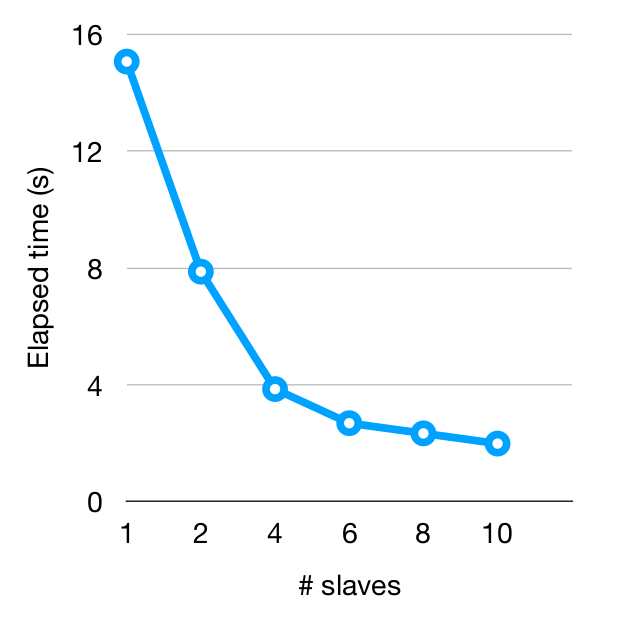
\includegraphics[width=0.6\textwidth]{appendix/exposure/ms_perf.png}
    \caption{
        Benchmarking of the serial and parallel code
        in the low level language.
    }
    \label{fig:parallel_benchmark}
\end{figure}

The hardware used to benchmark is composed of 6 cores and 
12 threads. Figure \ref{fig:parallel_benchmark} shows the 
scalability of the code
in terms of the elapsed time which is exponentiall decreasing with
% in the exponential trends of the elapsed time and
the number of slave processes.
The plateau curve on the edge is from the fact that
the maximum available running threads on this hardware
are only twelve which means that more workers that 
exceeds this limit do not reduce the computation time.
However, the total CPU cores on the cluster in space
physics laboratory are around 200 thread executors.
The performance from running the parallel code in the cluster 
takes only about twelve hours to finish.


